\documentclass[11pt,a4paper]{article}
\usepackage[T1]{fontenc}
\usepackage{lmodern}
\usepackage{geometry}
\geometry{margin=24mm}
\usepackage{microtype}
\usepackage{amsmath,amssymb}
\usepackage{booktabs,longtable,array}
\usepackage{enumitem}
\usepackage{xcolor}
\usepackage{listings}
\usepackage{tikz}
\usetikzlibrary{arrows.meta,positioning,shapes.geometric,calc}
\usepackage{hyperref}
\usepackage{fancyhdr}
\usepackage{caption}
\usepackage{float}
\usepackage{parskip}

\definecolor{codebg}{RGB}{247,248,250}
\definecolor{codeframe}{RGB}{210,214,220}
\definecolor{commentgreen}{RGB}{0,110,70}
\definecolor{keywordblue}{RGB}{20,70,160}
\definecolor{stringred}{RGB}{150,30,30}

\lstdefinestyle{cstyle}{
  language=C,
  basicstyle=\ttfamily\small,
  keywordstyle=\color{keywordblue}\bfseries,
  commentstyle=\color{commentgreen}\itshape,
  stringstyle=\color{stringred},
  backgroundcolor=\color{codebg},
  frame=single,
  rulecolor=\color{codeframe},
  numbers=left,
  numberstyle=\tiny\color{gray},
  stepnumber=1,
  numbersep=8pt,
  showstringspaces=false,
  tabsize=4,
  breaklines=true,
  columns=fullflexible,
  keepspaces=true,
  captionpos=b
}

\pagestyle{fancy}
\fancyhf{}
\lhead{SmartSafe Project}
\rhead{Power-Failure Detection Module}
\cfoot{\thepage}
\setlength{\headheight}{14pt}

\hypersetup{
  colorlinks=true,
  linkcolor=blue!60!black,
  urlcolor=blue!60!black,
  pdftitle={SmartSafe Power-Failure Detection Module},
  pdfauthor={SmartSafe Project Report}
}

\title{\textbf{SmartSafe Master Unit}\\[4pt]
\Large Complete Design and Code Explanation of the Power-Failure Detection Module}
\author{Microprocessors End-Term Project}
\date{July 2026}

\begin{document}
\maketitle
\thispagestyle{empty}

\begin{abstract}
This report documents the power-monitoring subsystem used in the SmartSafe Master unit. The module detects a simulated reduction of a monitored supply with the ATmega32 analog comparator, rejects short disturbances with a software stability filter, reports accepted power-state transitions to the main program, cooperates with two different sleep strategies, and correctly handles a failure already present at startup. The explanation follows the supplied \texttt{power.c} implementation and covers the external voltage divider, comparator polarity, register configuration, interrupt behavior, atomic sections, startup synchronization, normal inactivity sleep, power-failure standby, restoration handling, timing constants, and the interaction between the interrupt service routine, Timer2, and the main loop.
\end{abstract}

\tableofcontents
\newpage

\section{Purpose and Design Requirements}
The power module has four responsibilities:
\begin{enumerate}[label=\arabic*.]
  \item Monitor a separate adjustable voltage representing the Master supply.
  \item Detect a persistent drop below a selected threshold rather than reacting to a short spike or comparator chatter.
  \item Report one logical event for each accepted transition: normal-to-failed and failed-to-normal.
  \item Cooperate with the Master power-management policy:
  \begin{itemize}
    \item normal inactivity uses Power-down sleep and permits only INT0 to wake the processor;
    \item a confirmed power failure uses a dedicated standby state in which the comparator remains available to detect restoration.
  \end{itemize}
\end{enumerate}

The module deliberately separates \emph{raw hardware state} from \emph{accepted software state}. The analog comparator may change immediately and may toggle several times around the threshold. The rest of the application sees a transition only after the state remains stable for the configured confirmation interval.

\section{Hardware Arrangement}

\subsection{Comparator inputs}
With \texttt{ACBG=1}, the internal bandgap reference is connected to the non-inverting comparator input, denoted $V_+$. The divided monitored voltage is connected to \texttt{PB3/AIN1}, the inverting input $V_-$. The polarity is therefore:
\[
ACO = 1 \quad \Longleftrightarrow \quad V_+ > V_- \quad \Longleftrightarrow \quad V_{BG} > V_{AIN1}.
\]
The firmware interprets \texttt{ACO=1} as a power failure.

\begin{figure}[H]
\centering
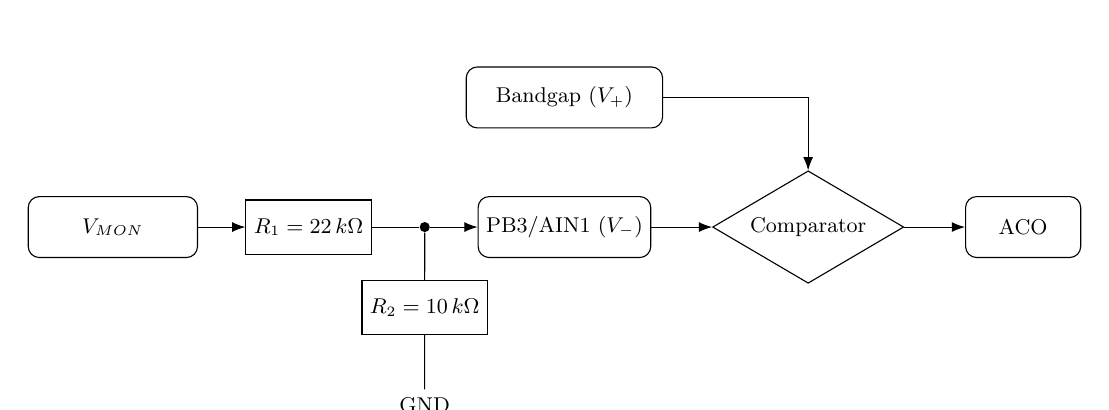
\begin{tikzpicture}[>=Latex, node distance=7mm, scale=0.86, transform shape, every node/.style={font=\small}]
  \node (vmon) [draw, rounded corners, minimum width=25mm, minimum height=9mm] {$V_{MON}$};
  \node (r1) [draw, right=of vmon, minimum width=18mm, minimum height=8mm] {$R_1=22\,k\Omega$};
  \node (mid) [circle, fill=black, inner sep=1.5pt, right=of r1] {};
  \node (ain) [draw, rounded corners, right=of mid, minimum width=24mm, minimum height=9mm] {PB3/AIN1 ($V_-$)};
  \node (r2) [draw, below=of mid, minimum width=18mm, minimum height=8mm] {$R_2=10\,k\Omega$};
  \node (gnd) [below=8mm of r2] {GND};
  \node (bg) [draw, rounded corners, above=10mm of ain, minimum width=29mm, minimum height=9mm] {Bandgap ($V_+$)};
  \node (comp) [draw, diamond, aspect=1.7, right=9mm of ain, minimum width=25mm] {Comparator};
  \node (aco) [draw, rounded corners, right=9mm of comp, minimum width=17mm, minimum height=9mm] {ACO};
  \draw[->] (vmon) -- (r1);
  \draw (r1) -- (mid);
  \draw[->] (mid) -- (ain);
  \draw (mid) -- (r2);
  \draw (r2) -- (gnd);
  \draw[->] (ain) -- (comp);
  \draw[->] (bg) -| (comp);
  \draw[->] (comp) -- (aco);
\end{tikzpicture}
\caption{Power-monitoring voltage divider and comparator polarity.}
\end{figure}

\subsection{Divider threshold}
The divider output is
\[
V_{AIN1}=V_{MON}\frac{R_2}{R_1+R_2}.
\]
For $R_1=22\,k\Omega$ and $R_2=10\,k\Omega$,
\[
V_{AIN1}=0.3125\,V_{MON}.
\]
The comparator changes state when $V_{AIN1}$ is approximately equal to the bandgap voltage. Using a nominal bandgap value of $1.23$ V,
\[
V_{MON,trip}=1.23\frac{22+10}{10}\approx3.94\text{ V}.
\]
Thus a nominal 5 V monitored source is treated as normal, while a reduction below roughly 4 V is treated as a failure. The exact point depends on the comparator model, bandgap tolerance, resistor tolerance, and simulation behavior.

\section{Module State Variables}

\begin{lstlisting}[style=cstyle,caption={Power-state variables.}]
volatile uint8_t power_event_pending = 0;
volatile uint8_t power_fail_state = 0;

static volatile uint8_t power_candidate_state = 0;
static volatile uint8_t power_confirm_ticks = 0;
static volatile uint8_t power_confirmation_pending = 0;
\end{lstlisting}

\begin{longtable}{>{\ttfamily}p{0.31\textwidth}p{0.61\textwidth}}
\toprule
\normalfont Variable & Meaning \\
\midrule
\endhead
power\_fail\_state & Last accepted and software-filtered state. Zero means normal power; one means failed power. This is the authoritative state used by the application. \\
power\_event\_pending & Notification flag for \texttt{main.c}. It becomes one when a new accepted state must be processed. \\
power\_candidate\_state & Raw comparator state captured by the latest comparator transition. \\
power\_confirm\_ticks & Remaining 10 ms intervals before the candidate may be accepted. \\
power\_confirmation\_pending & Indicates that a candidate is currently being verified. \\
\bottomrule
\end{longtable}

The accepted state and event flag are \texttt{volatile} because they are shared between the module and the application. The filter variables are also \texttt{volatile} because the comparator ISR and Timer2 ISR modify them while the main loop reads them.

\section{Reading the Comparator Output}

\begin{lstlisting}[style=cstyle,caption={Conversion of ACO into a logical failure state.}]
static uint8_t comparator_reports_power_fail(void)
{
    return (ACSR & (1 << ACO)) ? 1U : 0U;
}
\end{lstlisting}

This helper isolates the hardware polarity from the rest of the code. A return value of one always means ``power failed,'' even though the actual hardware condition is ``the bandgap input is greater than the divided monitored input.'' This improves readability and avoids repeated direct interpretation of \texttt{ACO}.

\section{Analog Comparator Register Configuration}
The ATmega32 Analog Comparator Control and Status Register, \texttt{ACSR}, contains the fields shown below.

\begin{table}[H]
\centering
\caption{ACSR fields relevant to the project.}
\begin{tabular}{clp{0.57\textwidth}}
\toprule
Bit & Name & Project use \\
\midrule
7 & ACD & Comparator disable. Kept at zero so the comparator remains powered. \\
6 & ACBG & Internal bandgap select. Set to one, connecting the bandgap to $V_+$. \\
5 & ACO & Read-only comparator output. One is interpreted as failure. \\
4 & ACI & Comparator interrupt flag. It is cleared by writing a logic one. \\
3 & ACIE & Comparator interrupt enable. Set while transitions must generate interrupts. \\
2 & ACIC & Timer1 input-capture connection. Kept at zero. \\
1:0 & ACIS1:0 & Interrupt mode. Both remain zero, selecting interrupt on comparator-output toggle. \\
\bottomrule
\end{tabular}
\end{table}

The code intentionally uses complete assignments such as
\begin{lstlisting}[style=cstyle]
ACSR = (1 << ACBG) | (1 << ACI);
ACSR = (1 << ACBG) | (1 << ACIE);
\end{lstlisting}
rather than read-modify-write operations. This matters because \texttt{ACI} is a write-one-to-clear flag. Writing zero leaves it unchanged; writing one clears it. An expression such as \texttt{ACSR \&= \textasciitilde(1<<ACI)} would not clear the flag.

\subsection{Dedicated AIN1 rather than ADC multiplexer input}
The comparator can optionally use the ADC multiplexer as its negative input when \texttt{ACME} is enabled under the required ADC conditions. This design uses the dedicated \texttt{AIN1/PB3} pin, so the code clears \texttt{ACME}:
\begin{lstlisting}[style=cstyle]
#ifdef ACME
    SFIOR &= ~(1U << ACME);
#endif
\end{lstlisting}
This avoids accidental routing of an ADC channel into the comparator.

\section{Initialization Sequence}

\begin{lstlisting}[style=cstyle,caption={Power-monitor initialization.}]
void power_monitor_init(void)
{
    uint8_t initial_state;

    POWER_SENSE_DDR &= ~(1U << POWER_SENSE_PIN);
    POWER_SENSE_PORT &= ~(1U << POWER_SENSE_PIN);

#ifdef ACME
    SFIOR &= ~(1U << ACME);
#endif

    ACSR = (1U << ACBG);
    delay_ms(1);

    initial_state = comparator_reports_power_fail();

    power_fail_state = initial_state;
    power_candidate_state = initial_state;
    power_event_pending = initial_state ? 1U : 0U;

    power_confirm_ticks = 0;
    power_confirmation_pending = 0;

    ACSR = (1U << ACBG) | (1U << ACI);
    ACSR = (1U << ACBG) | (1U << ACIE);
}
\end{lstlisting}

\subsection{Pin direction and pull-up}
The power-sense pin is configured as an input and its pull-up is disabled:
\begin{lstlisting}[style=cstyle]
POWER_SENSE_DDR  &= ~(1U << POWER_SENSE_PIN);
POWER_SENSE_PORT &= ~(1U << POWER_SENSE_PIN);
\end{lstlisting}
The external divider already defines the voltage. Enabling the internal pull-up would alter the divider ratio and move the detection threshold.

\subsection{Bandgap stabilization}
The comparator is first enabled with its interrupt disabled:
\begin{lstlisting}[style=cstyle]
ACSR = (1U << ACBG);
delay_ms(1);
\end{lstlisting}
The delay allows the internal reference and simulated comparator model to settle before the initial state is read. A 1 ms delay is intentionally conservative relative to the hardware startup requirement.

\subsection{Failure already present at startup}
After the delay, the raw state is copied into both the accepted state and candidate state. If it is already failed, \texttt{power\_event\_pending} is set immediately:
\begin{lstlisting}[style=cstyle]
power_event_pending = initial_state ? 1U : 0U;
\end{lstlisting}
This is essential because a comparator interrupt is generated by a transition. If the voltage was already low at reset, no new edge may occur. The startup event ensures that the main loop still sends and logs the failure and enters the correct standby mode.

\section{Comparator Interrupt Service Routine}

\begin{lstlisting}[style=cstyle,caption={Comparator ISR.}]
ISR(ANA_COMP_vect)
{
    power_candidate_state = comparator_reports_power_fail();
    power_confirm_ticks = POWER_CONFIRM_TICKS_10MS;
    power_confirmation_pending = 1;
}
\end{lstlisting}

The ISR is intentionally short. It does not send USART text, write EEPROM, update the LCD, or enter sleep. It only captures the raw state and restarts the confirmation interval. Heavy operations inside an ISR would increase latency, complicate nested timing, and risk blocking other interrupt-driven functions.

With \texttt{ACIS1:ACIS0=00}, the interrupt occurs when \texttt{ACO} toggles:
\[
0\rightarrow1 \quad\text{or}\quad 1\rightarrow0.
\]
A stable normal voltage does not repeatedly invoke the ISR. A stable failed voltage also does not repeatedly invoke it. Only threshold crossings or chatter create interrupts.

\section{Software Stability Filter}

\subsection{Confirmation time constant}
The project constant is
\begin{lstlisting}[style=cstyle]
#define POWER_CONFIRM_TICKS_10MS 10U
\end{lstlisting}
Timer2 calls \texttt{power\_monitor\_tick\_10ms()} approximately every 10 ms. Ten ticks correspond to approximately 100 ms:
\[
10\times9.984\text{ ms}\approx99.84\text{ ms}.
\]
This rejects short switching transients and manually induced noise without making the system feel slow.

\subsection{Timer2-side countdown}

\begin{lstlisting}[style=cstyle]
void power_monitor_tick_10ms(void)
{
    if (power_confirmation_pending && power_confirm_ticks > 0)
        power_confirm_ticks--;
}
\end{lstlisting}

The function is designed to be called from the Timer2 compare ISR. It performs only a bounded decrement. When the counter reaches zero, the candidate becomes eligible for main-loop validation.

\subsection{Main-loop acceptance}

\begin{lstlisting}[style=cstyle,caption={Candidate validation and acceptance.}]
void power_monitor_process(void)
{
    uint8_t candidate;
    uint8_t sreg;

    sreg = SREG;
    cli();

    if (!power_confirmation_pending || power_confirm_ticks != 0) {
        SREG = sreg;
        return;
    }

    candidate = power_candidate_state;
    power_confirmation_pending = 0;

    SREG = sreg;

    if (comparator_reports_power_fail() != candidate)
        return;

    if (candidate != power_fail_state) {
        power_fail_state = candidate;
        power_event_pending = 1;
    }
}
\end{lstlisting}

The atomic section prevents the comparator ISR or Timer2 ISR from changing the candidate and countdown while the main loop is deciding whether the interval has completed. Interrupts are restored to their previous state by writing back the saved \texttt{SREG}; the code does not assume that interrupts were enabled before entry.

After leaving the atomic section, the function reads the live comparator again. A candidate is rejected if the hardware no longer agrees. Finally, an event is produced only when the accepted state actually changes. This prevents duplicate events for the same stable condition.

\begin{figure}[H]
\centering
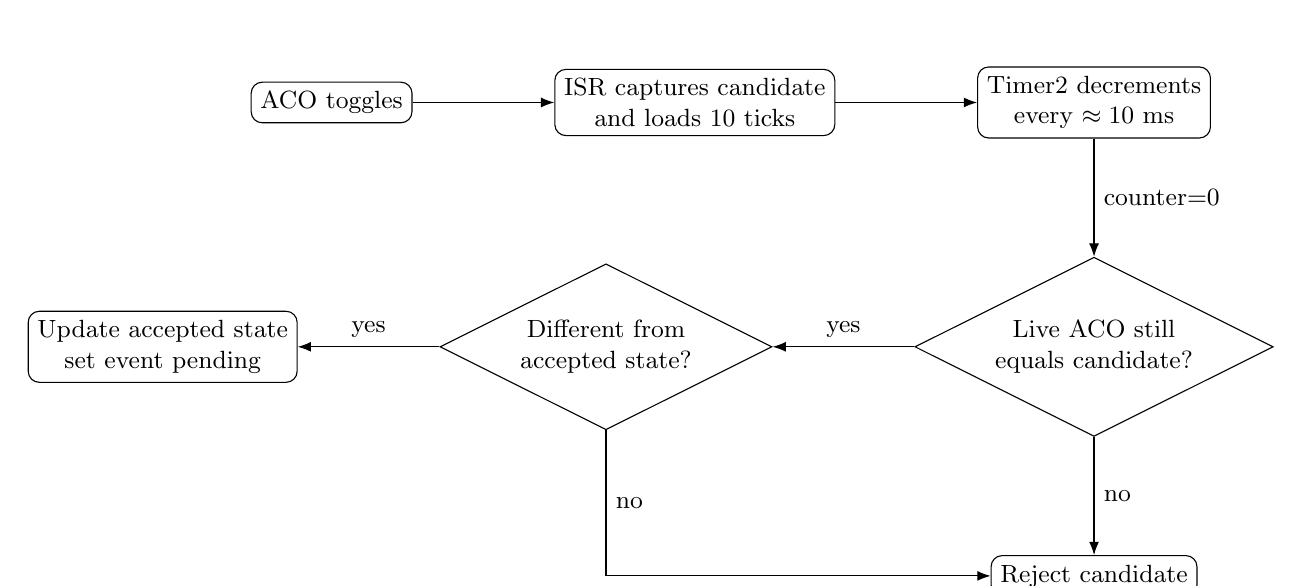
\begin{tikzpicture}[node distance=15mm and 18mm, >=Latex, every node/.style={font=\small, align=center}]
\node (edge) [draw, rounded corners] {ACO toggles};
\node (isr) [draw, rounded corners, right=of edge] {ISR captures candidate\\and loads 10 ticks};
\node (count) [draw, rounded corners, right=of isr] {Timer2 decrements\\every $\approx10$ ms};
\node (live) [draw, diamond, aspect=2, below=of count] {Live ACO still\\equals candidate?};
\node (same) [draw, diamond, aspect=2, left=of live] {Different from\\accepted state?};
\node (event) [draw, rounded corners, left=of same] {Update accepted state\\set event pending};
\node (reject) [draw, rounded corners, below=of live] {Reject candidate};
\draw[->] (edge) -- (isr);
\draw[->] (isr) -- (count);
\draw[->] (count) -- node[right]{counter=0} (live);
\draw[->] (live) -- node[above]{yes} (same);
\draw[->] (live) -- node[right]{no} (reject);
\draw[->] (same) -- node[above]{yes} (event);
\draw[->] (same) |- node[pos=0.25,right]{no} (reject);
\end{tikzpicture}
\caption{Temporal filtering and accepted-state transition logic.}
\end{figure}

\section{Interaction with the Main Loop}
The main loop repeatedly performs two operations:
\begin{lstlisting}[style=cstyle]
power_monitor_process();
process_power_event();
\end{lstlisting}
The first accepts a stable candidate. The second, implemented in the application layer, consumes \texttt{power\_event\_pending}. On failure it typically:
\begin{enumerate}
  \item clears the pending flag;
  \item sends \texttt{POWER\_FAIL} through USART;
  \item waits for the final USART stop bit if necessary;
  \item writes \texttt{EVT\_POWER\_FAIL} to the external EEPROM;
  \item turns off or disables nonessential Master peripherals;
  \item enters the dedicated restoration-wait state.
\end{enumerate}
On restoration it sends \texttt{POWER RESTORED}, logs \texttt{EVT\_POWER\_OK}, reinitializes disabled peripherals, and returns to normal operation.

\section{Normal Inactivity Sleep}
Normal inactivity sleep uses Power-down mode and intentionally permits only INT0 to wake the Master. The comparator interrupt is therefore suspended before sleep.

\subsection{Suspending comparator events}

\begin{lstlisting}[style=cstyle]
void power_monitor_suspend_for_sleep(void)
{
    uint8_t sreg = SREG;
    cli();

    power_confirm_ticks = 0;
    power_confirmation_pending = 0;

    ACSR = (1 << ACBG) | (1 << ACI);

    SREG = sreg;
}
\end{lstlisting}

The function cancels an unfinished candidate and clears any stale comparator interrupt flag. Because \texttt{ACIE} is omitted from the assignment, comparator interrupts are disabled. The comparator itself remains enabled because \texttt{ACBG} is retained and \texttt{ACD} remains zero.

\subsection{Resynchronizing after INT0 wake}

\begin{lstlisting}[style=cstyle]
void power_monitor_resume_after_sleep(void)
{
    uint8_t current;
    uint8_t sreg;

    ACSR = (1 << ACBG) | (1 << ACI);
    ACSR = (1 << ACBG) | (1 << ACIE);

    current = comparator_reports_power_fail();

    sreg = SREG;
    cli();

    if (current != power_fail_state) {
        power_candidate_state = current;
        power_confirm_ticks = POWER_CONFIRM_TICKS_10MS;
        power_confirmation_pending = 1;
    } else {
        power_candidate_state = current;
        power_confirm_ticks = 0;
        power_confirmation_pending = 0;
    }

    SREG = sreg;
}
\end{lstlisting}

Power may have changed while the MCU was asleep, but that change was not allowed to wake it. After INT0 wakes the Master, the module reads the current comparator state. If it differs from the accepted state, the ordinary 100 ms confirmation process is restarted. No event is lost merely because the comparator interrupt was disabled during Power-down.

\section{Power-Failure Standby and Restoration}
The confirmed power-failure state is different from normal inactivity sleep. The Master has already sent and logged the failure. It disables nonessential peripherals, but the comparator must remain capable of detecting restoration.

\subsection{Preparing for restoration}

\begin{lstlisting}[style=cstyle]
void power_monitor_prepare_restore_wait(void)
{
    uint8_t sreg = SREG;
    cli();

    power_candidate_state = 1U;
    power_confirm_ticks = 0;
    power_confirmation_pending = 0;

    ACSR = (1 << ACBG) | (1 << ACI);
    ACSR = (1 << ACBG) | (1 << ACIE);

    SREG = sreg;
}
\end{lstlisting}

The failure has already been accepted, so the filter is cleared. The comparator interrupt is re-enabled in toggle mode. In the surrounding standby code, other interrupt sources are disabled, and the MCU uses a sleep mode from which the comparator can wake it.

\subsection{Raw state check}

\begin{lstlisting}[style=cstyle]
uint8_t power_monitor_raw_failed(void)
{
    return comparator_reports_power_fail();
}
\end{lstlisting}

This function is used by the standby loop to decide whether the failed condition still exists before sleeping again. It intentionally bypasses the normal 100 ms filter because Timer2 is stopped in the reduced-power state.

\subsection{Accepting restoration}

\begin{lstlisting}[style=cstyle]
uint8_t power_monitor_accept_restore_if_present(void)
{
    uint8_t restored = 0;
    uint8_t sreg = SREG;

    cli();

    if (!comparator_reports_power_fail()) {
        power_fail_state = 0;
        power_event_pending = 1;
        power_candidate_state = 0;
        power_confirm_ticks = 0;
        power_confirmation_pending = 0;
        restored = 1;
    }

    SREG = sreg;
    return restored;
}
\end{lstlisting}

Restoration is accepted atomically when the raw comparator reports normal power. The accepted state is changed to zero and an event is queued for the application. The return value allows the standby loop to break and reinitialize the runtime peripherals.

This restoration path is intentionally immediate rather than temporally filtered because the 10 ms Timer2 time base is stopped during standby. The trade-off is greater sensitivity to chatter during restoration. In a physical design, hardware hysteresis or a short dedicated confirmation method can be added if required.

\section{Two Sleep Policies}

\begin{table}[H]
\centering
\caption{Comparison of the two Master sleep conditions.}
\begin{tabular}{p{0.26\textwidth}p{0.32\textwidth}p{0.32\textwidth}}
\toprule
Characteristic & Normal inactivity sleep & Confirmed power-failure standby \\
\midrule
Purpose & Save power after about 10 seconds without activity & Simulate a Master that shuts down most functions after supply failure \\
Typical mode & Power-down & Idle or another comparator-wake-capable state used by the application \\
Allowed wake source & INT0 only & Analog comparator restoration transition \\
Comparator interrupt & Disabled before sleep & Enabled \\
Timer2 & Stopped by Power-down & Explicitly stopped by standby setup \\
Power change while asleep & Detected only after INT0 wake and resynchronization & Restoration wakes the processor \\
\bottomrule
\end{tabular}
\end{table}

\section{Concurrency and Atomicity}
The module shares 8-bit variables among the main loop and two ISRs. Although individual 8-bit reads and writes are atomic on an 8-bit AVR, multi-step decisions are not. For example, the main loop must not observe \texttt{power\_confirmation\_pending=1}, then be interrupted while checking \texttt{power\_confirm\_ticks}, and continue with a different candidate. Saving \texttt{SREG}, executing \texttt{cli()}, and restoring \texttt{SREG} creates a short consistent snapshot without unconditionally enabling interrupts.

The ISR itself remains minimal, while slow operations such as EEPROM writes and USART transmission remain in the main context. This division is central to reliable embedded design.

\section{Expected Operating Sequences}

\subsection{Normal-to-failed transition}
\begin{enumerate}
  \item $V_{MON}$ falls until $V_{AIN1}<V_{BG}$.
  \item \texttt{ACO} changes from zero to one.
  \item The comparator ISR captures candidate state one and loads ten confirmation ticks.
  \item Timer2 decrements the counter for approximately 100 ms.
  \item The main loop verifies that the live comparator is still failed.
  \item The accepted state changes from zero to one and \texttt{power\_event\_pending} becomes one.
  \item The application sends the remote message, logs the event, disables peripherals, and enters restoration standby.
\end{enumerate}

\subsection{Failed-to-normal transition}
\begin{enumerate}
  \item $V_{MON}$ rises until $V_{AIN1}>V_{BG}$.
  \item \texttt{ACO} toggles to zero and wakes the MCU from power-failure standby.
  \item The standby loop confirms that the raw failed condition is no longer present.
  \item \texttt{power\_monitor\_accept\_restore\_if\_present()} changes the accepted state to normal and queues an event.
  \item Runtime peripherals are reinitialized.
  \item The application sends and logs the restoration event.
\end{enumerate}

\subsection{Reset while voltage is already low}
\begin{enumerate}
  \item The MCU resets and calls \texttt{power\_monitor\_init()}.
  \item The bandgap is enabled and allowed to settle for 1 ms.
  \item The initial comparator state is read as failed.
  \item \texttt{power\_event\_pending} is set even though no transition occurred.
  \item The application immediately processes the existing failure and returns to standby.
\end{enumerate}

\section{Diagnostic Checks in Proteus}
Useful logic and voltage probes are:
\begin{itemize}
  \item a voltmeter at the potentiometer output $V_{MON}$;
  \item a voltmeter at \texttt{PB3/AIN1};
  \item a logic probe for a temporary application debug pin when an accepted event is processed;
  \item the Virtual Terminal to observe \texttt{POWER\_FAIL} and \texttt{POWER RESTORED};
  \item a watch on \texttt{ACO}, \texttt{power\_candidate\_state}, \texttt{power\_confirm\_ticks}, and \texttt{power\_fail\_state}.
\end{itemize}

At a normal monitored voltage of 5 V, the intended divider should produce approximately 1.56 V on AIN1. At the nominal trip point, AIN1 should be close to the comparator reference. If the observed monitored-voltage trip point is very different, both the source voltage and divider midpoint must be measured before changing resistor values.

\section{Design Strengths and Limitations}
\subsection{Strengths}
\begin{itemize}
  \item The comparator ISR is short and deterministic.
  \item Startup failure is handled without requiring an edge.
  \item Temporal filtering rejects short disturbances.
  \item Accepted-state tracking prevents repeated duplicate events.
  \item Sleep integration preserves the requirement that INT0 is the only normal Power-down wake source.
  \item Complete \texttt{ACSR} assignments correctly handle the write-one-to-clear \texttt{ACI} flag.
\end{itemize}

\subsection{Limitations}
\begin{itemize}
  \item The comparator threshold depends on bandgap and resistor tolerances.
  \item There is no hardware hysteresis; continuous noise near the threshold can repeatedly restart confirmation.
  \item Restoration during power-failure standby is accepted without the 100 ms filter because Timer2 is stopped.
  \item The simulation keeps the MCU supply alive while varying a separate monitored voltage; it does not model a true capacitor-backed last-gasp shutdown.
\end{itemize}

\section{Complete Module Listing}
The following listing is the supplied power module used as the basis of this report.

\begin{lstlisting}[style=cstyle,caption={Complete power.c implementation.}]
#include <avr/io.h>
#include <avr/interrupt.h>
#include "config.h"
#include "power.h"
#include "timer.h"

volatile uint8_t power_event_pending = 0;
volatile uint8_t power_fail_state = 0;

static volatile uint8_t power_candidate_state = 0;
static volatile uint8_t power_confirm_ticks = 0;
static volatile uint8_t power_confirmation_pending = 0;

static uint8_t comparator_reports_power_fail(void)
{
    return (ACSR & (1 << ACO)) ? 1U : 0U;
}

ISR(ANA_COMP_vect)
{
    power_candidate_state = comparator_reports_power_fail();
    power_confirm_ticks = POWER_CONFIRM_TICKS_10MS;
    power_confirmation_pending = 1;
}

void power_monitor_tick_10ms(void)
{
    if (power_confirmation_pending && power_confirm_ticks > 0)
        power_confirm_ticks--;
}

void power_monitor_process(void)
{
    uint8_t candidate;
    uint8_t sreg;

    sreg = SREG;
    cli();

    if (!power_confirmation_pending || power_confirm_ticks != 0) {
        SREG = sreg;
        return;
    }

    candidate = power_candidate_state;
    power_confirmation_pending = 0;

    SREG = sreg;

    if (comparator_reports_power_fail() != candidate)
        return;

    if (candidate != power_fail_state) {
        power_fail_state = candidate;
        power_event_pending = 1;
    }
}

void power_monitor_suspend_for_sleep(void)
{
    uint8_t sreg = SREG;
    cli();

    power_confirm_ticks = 0;
    power_confirmation_pending = 0;

    ACSR = (1 << ACBG) | (1 << ACI);

    SREG = sreg;
}

void power_monitor_resume_after_sleep(void)
{
    uint8_t current;
    uint8_t sreg;

    ACSR = (1 << ACBG) | (1 << ACI);
    ACSR = (1 << ACBG) | (1 << ACIE);

    current = comparator_reports_power_fail();

    sreg = SREG;
    cli();

    if (current != power_fail_state) {
        power_candidate_state = current;
        power_confirm_ticks = POWER_CONFIRM_TICKS_10MS;
        power_confirmation_pending = 1;
    } else {
        power_candidate_state = current;
        power_confirm_ticks = 0;
        power_confirmation_pending = 0;
    }

    SREG = sreg;
}

void power_monitor_prepare_restore_wait(void)
{
    uint8_t sreg = SREG;
    cli();

    power_candidate_state = 1U;
    power_confirm_ticks = 0;
    power_confirmation_pending = 0;

    ACSR = (1 << ACBG) | (1 << ACI);
    ACSR = (1 << ACBG) | (1 << ACIE);

    SREG = sreg;
}

uint8_t power_monitor_raw_failed(void)
{
    return comparator_reports_power_fail();
}

uint8_t power_monitor_accept_restore_if_present(void)
{
    uint8_t restored = 0;
    uint8_t sreg = SREG;

    cli();

    if (!comparator_reports_power_fail()) {
        power_fail_state = 0;
        power_event_pending = 1;
        power_candidate_state = 0;
        power_confirm_ticks = 0;
        power_confirmation_pending = 0;
        restored = 1;
    }

    SREG = sreg;
    return restored;
}

void power_monitor_init(void)
{
    uint8_t initial_state;

    POWER_SENSE_DDR &= ~(1U << POWER_SENSE_PIN);
    POWER_SENSE_PORT &= ~(1U << POWER_SENSE_PIN);

#ifdef ACME
    SFIOR &= ~(1U << ACME);
#endif

    ACSR = (1U << ACBG);
    delay_ms(1);

    initial_state = comparator_reports_power_fail();

    power_fail_state = initial_state;
    power_candidate_state = initial_state;
    power_event_pending = initial_state ? 1U : 0U;

    power_confirm_ticks = 0;
    power_confirmation_pending = 0;

    ACSR = (1U << ACBG) | (1U << ACI);
    ACSR = (1U << ACBG) | (1U << ACIE);
}
\end{lstlisting}

\section{Conclusion}
The power module is a small event-driven state machine built on the ATmega32 analog comparator. Hardware detects threshold crossings immediately; a 100 ms software filter converts noisy raw transitions into stable application events. The design also distinguishes two power-management contexts: comparator-disabled normal Power-down sleep and comparator-enabled restoration standby. Startup synchronization, write-one-to-clear flag handling, atomic state updates, and separation of ISR work from main-loop work are the key implementation details that make the module dependable.

\begin{thebibliography}{9}
\bibitem{atmega32}
Microchip Technology, \emph{ATmega32/L Datasheet}, Analog Comparator, I/O Ports, Interrupts, and Sleep Modes.\\
\url{https://ww1.microchip.com/downloads/en/DeviceDoc/doc2503.pdf}

\bibitem{project}
SmartSafe Microprocessors End-Term Project Specification, Spring 1404.
\end{thebibliography}

\end{document}
